\chapter{Trabalhos Relacionados}

No trabalho \textit{Multi-agent system testing: A survey} \citet{houhamdi2011multi} faz uma investigação e descreve os trabalhos relacionados ao tema de teste em agentes. A separação em níveis de teste facilita a compreensão, também acontecem de alguns trabalhos citados ocuparem mais de um nível de teste. A Tabela \ref{tab:trabalhos_teste} mostra a relação de trabalhos apresentadas neste artigo e seus respectivos níveis. Mais detalhes sobre cada nível de teste pode ser visto na sessão \ref{sec:testesma}.

O autor conclui que os trabalhos em testes em SMA se concentram principalmente no nível de agente e integração e expões áreas de investigações de teste que necessitam de atenção como: desenvolver um processo de teste completo para SMA, testes no nível de aceitação, testar propriedades emergentes no nível de sistema macroscópico, métricas para avaliar a qualidade dos testes em SMA e reduzir ou remover os efeitos colaterais na execução e monitoramento dos testes.

\begin{table}[ht]
\centering
\caption{Relação entre níveis de teste e trabalhos relacionados \cite{houhamdi2011multi}.}
\label{tab:trabalhos_teste}
\begin{tabular}{@{}lcl@{}}
\toprule
Tipo de Teste                        & Descrição                                                                                                                          & Trabalhos                   \\ \midrule
\multirow{2}{*}{Teste de Unidade}    & \multirow{2}{*}{\makecell{Teste nos menores blocos \\ de construção de um SMA.}}                                                                   & \cite{zhang2007automated} \\ \cmidrule(l){3-3} 
                                     &                                                                                                                                    & \cite{ekinci2009goal}                   \\ \midrule
\multirow{6}{*}{Teste do Agente}     & \multirow{6}{*}{\makecell{Teste de integração \\ dos diferentes módulos \\ dos agentes.}}                                                           & \cite{caire2004multi}                   \\ \cmidrule(l){3-3} 
                                     &                                                                                                                                    & \cite{lam2004debugging}                   \\ \cmidrule(l){3-3} 
                                     &                                                                                                                                    & \cite{nunez2005specification}                   \\ \cmidrule(l){3-3} 
                                     &                                                                                                                                    & \cite{coelho2006unit}                   \\ \cmidrule(l){3-3} 
                                     &                                                                                                                                    & \cite{gomez2008testing}                   \\ \cmidrule(l){3-3} 
                                     &                                                                                                                                    & \cite{houhamdi2011multi}                   \\ \midrule
\multirow{7}{*}{Teste de Integração} & \multirow{7}{*}{\makecell{Testa a interação entre \\ agentes e a interação destes \\com o ambiente.}} & \cite{knublauch2002extreme}                   \\ \cmidrule(l){3-3} 
                                     &                                                                                                                                    & \cite{botia2004aclanalyser}                   \\ \cmidrule(l){3-3} 
                                     &                                                                                                                                    & \cite{padgham2005adding}                   \\ \cmidrule(l){3-3} 
                                     &                                                                                                                                    & \cite{rodrigues2005towards}                   \\ \cmidrule(l){3-3} 
                                     &                                                                                                                                    & \cite{ekinci2009goal}                   \\ \cmidrule(l){3-3} 
                                     &                                                                                                                                    & \cite{nguyen2009goal}                   \\ \cmidrule(l){3-3} 
                                     &                                                                                                                                    & \cite{houhamdi2011structured}                   \\ \midrule
\multirow{2}{*}{Teste de Sistema}    & \multirow{2}{*}{\makecell{Testa o SMA no \\ ambiente de operação. }}                                                                                                       & \cite{sudeikat2008systemic}                   \\ \cmidrule(l){3-3} 
                                     &                                                                                                                                    & \cite{houhamdi2011structured}                   \\ \midrule
                                     
\multirow{2}{*}{Teste de Aceitação}  & \multirow{2}{*}{\makecell{Verifica se atende aos \\objetivos do cliente.}}                                                                       & \multirow{2}{*}{Sem trabalhos relacionados} \\
                                     &                                                                                                                                    &                                             \\ \bottomrule
\end{tabular}
\end{table}


Em \cite{athamena2012petri} os autores propõem uma abordagem baseada em RP pra o teste de comportamento de SMA. Para isso modelos de análise e projeto criados com base na metodologia MaSE são convertidos em um modelo UML 2.0 padrão, e então os modelos UML são transformados em RP para testes formais, a Figura \ref{fig:fluxograma} apresenta as atividades da abordagem.

\begin{figure}[ht]
\centering
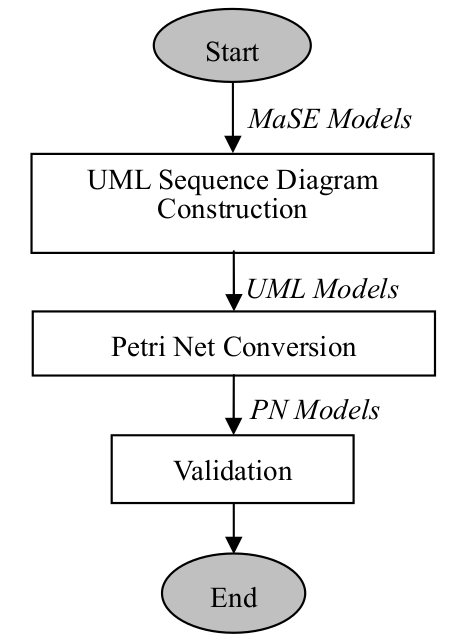
\includegraphics[scale=0.4]{imagens/fluxograma.png}
\caption{Fluxograma do projeto de teste no SMA \cite{athamena2012petri}.}
\label{fig:fluxograma}
\end{figure}

Neste trabalho os autores desenvolveram um modelo para a transformação dos diagrama de classe de agente e diagrama de função do MaSE, para o diagrama de sequência do modelo UML 2.0, e então propuseram um modelo para transformar os diagramas de sequencia em RP equivalentes e enfim podem ser aplicados as técnicas de testes automáticos no SMA.

Segundo os autores as principais contribuições do trabalhos foi propor um processo de teste completo e abrangente para o SMA e reduzir os efeitos colaterais na execução e monitoramento do teste, não utilizando agentes testadores ou agentes oráculos o que pode influenciar no comportamento dos agentes ou desempenho do sistema.


Em \cite{winikoff2014testability} o objetivo é avaliar o quão difícil é testar um programa de agente na arquitetura BDI. Para isso o autor utiliza a técnica de testes de caixa-branca que é baseada no fluxo de controle, um critério básico e muito longo para avaliar a adequação de um conjunto de testes em que todos os caminhos (\textit{All-Path}) do programa sejam cobertos. Um motivo pela escolha de utilizar todos os caminhos é que os SMA geralmente envolvem ambientes não-episódicos, sendo que o comportamento de um determinado plano ou meta é geralmente sensível ao histórico do agente, precisando assim considerar as diferentes histórias possíveis.

Neste trabalho para analisar o processo de execução BDI é utilizada uma visão declarativa. Os eventos e planos podem ser visualizados como uma árvore em que cada objetivo tem como filhos as instâncias do plano que são aplicáveis a ele, e cada instância do plano tem como filhos os sub-objetivos que ele publica. Esta forma de visualização facilita a análise do número de caminhos através de um programa BDI.

Para a geração de árvore um programa em Prolog foi implementado, onde uma árvore de plano-meta é representada por termos Prolog com a gramática apresentada na Figura \ref{fig:prolog} onde árvore de plano-meta (Goal-Plan Tree) é representado por GPT, o AoGL abreviou lista de ação ou meta (Action or Goal List) e A é um símbolo. Por exemplo a Figura \ref{fig:arvore} mostra a árvore de plano-meta simplificada modelada pelo termo Prolog \begin{math} goal\left ( \left [ plan\left ( \left [ act\left ( a \right ) \right ] \right ),plan\left ( \left [ act\left ( b \right ) \right ] \right ) \right ] \right )\end{math}.

%\begin{figure}
%  \centering
%  \subfigure[Prolog]{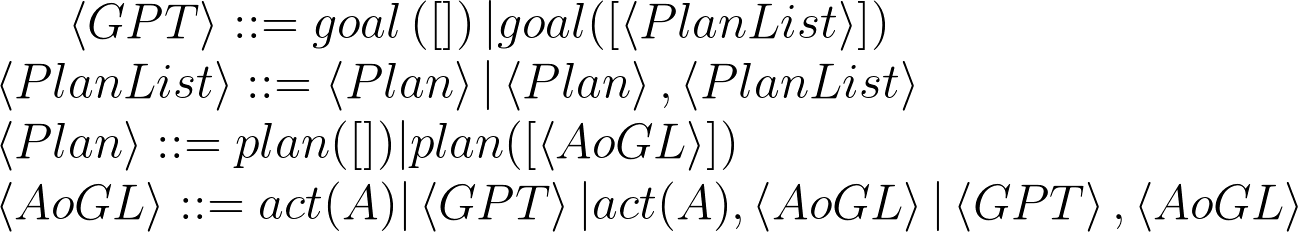
\includegraphics[width=0.6\textwidth]{imagens/code.png}\label{fig:prolog}}
%  \subfigure[Árvore]{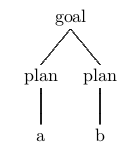
\includegraphics[width=0.2\textwidth]{imagens/simple_tree.png}\label{fig:arvore}}
%  \caption{COLOCAR UMA CAPTION AQUI}
%  \label{fig:prolog,arvore}
%\end{figure}


\begin{figure}[ht]
\centering
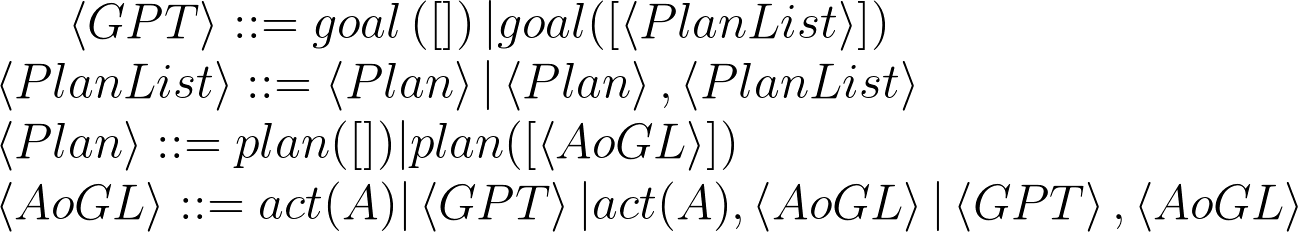
\includegraphics[scale=0.3]{imagens/code.png}
\caption{Termos Prolog \cite{winikoff2014testability}.}
\label{fig:prolog}
\end{figure}

\begin{figure}[ht]
\centering
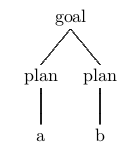
\includegraphics[scale=0.7]{imagens/simple_tree.png}
\caption{Árvore de plano-meta \cite{winikoff2014testability}.}
\label{fig:arvore}
\end{figure}




Com isso em vez de ver a execução de um programa BDI como um processo, o programa é visualizado como uma transformação de dados de uma árvore de planos-metas (finita) em uma sequencia de execuções de ações. Assim, a questão de quão grande é o espaço de comportamento para os agentes BDI é respondida derivando fórmulas que permitem calcular o número de comportamentos, bem-sucedidos e mal sucedidos (ou seja, falhou) para uma determinada planta de plano de meta.

Após testes em modelos de execução BDI abstratos os autores verificaram se os dados obtidos se aplicavam também à modelos reais. A aplicação real escolhida foi o trabalho de \cite{burmeister2008bdi} que preenchia os requisitos para a comparação. Os valores obtidos são apresentados na Tabela \ref{tab:result_ontestability} onde $n^{\checkmark}(g)$ são os caminhos que os testes são bem sucedidos, $n^{\upchi}(g)$ são os caminhos onde os teste falham e $\ell$ são ações antes, depois e entre sub-metas em um plano.

\begin{table}[ht]
\centering
\caption{Resultado do teste realizado em uma aplicação BDI \cite{winikoff2014testability}}
\label{tab:result_ontestability}
\begin{tabular}{@{}lllll@{}}
\toprule
\multirow{2}{*}{Árvore com 57 metas} & \multicolumn{2}{l}{Sem manipulação de Falha} & \multicolumn{2}{l}{Com manipulação de Falha}                  \\
                                        & $n^{\checkmark}(g)$     & $n^{\upchi}(g)$    & $n^{\checkmark}(g)$           & $n^{\upchi}(g)$               \\ \midrule
$\ell = 4$                              & 294,912                 & 3,250,604          & $\approx 2.98 \times 10^{20}$ & $\approx 9.69 \times 10^{20}$ \\
$\ell = 2$                              & 294,912                 & 1,625,302          & $\approx 6.28 \times 10^{15}$ & $\approx 8.96 \times 10^{15}$ \\
$\ell = 1$                              & 294,912                 & 812,651            & $\approx 9.66 \times 10^{11}$ & $\approx 6.27 \times 10^{11}$ \\ \bottomrule
\end{tabular}
\end{table}

Neste artigo os autores concluíram que um teste completo em um sistema BDI não é viável. O tamanho de espaços de comportamento é muito grande e ainda se torna significativamente maior quando o sistema tem suporte à manipulação de falhas. Os autores também chegaram à conclusão de que o mecanismo de recuperação de falhas é eficaz para alcançar uma baixa taxa de falha real. E novas abordagens foram propostas para lidar com a testabilidade do sistema.


O trabalho \cite{winikoff2017bdi} retorna com o objetivo de avaliar se é possível obter garantias em um sistema multiagente através de testes, verificando a testabilidade de um programa, dando continuidade no trabalho anterior \cite{winikoff2014testability}, mas utilizando novas métricas. A testabilidade de um programa é um métrica que indica o esforço necessário para testar adequadamente um programa. Este trabalho tem por objetivo quantificar quantos testes são necessários para testar um um programa de agente BDI para satisfazer um critério considerando o critério de adequação do teste de todas as arestas, que é considerado como o mínimo geralmente aceito \cite{jorgensen2016software}. 

Uma das grandes contribuições dos autores é que a  análise é genérica permitindo a aplicação a todos os programas que utilizam a arquitetura BDI. Para esta análise equações são derivadas  para chegar a conclusão de quantos casos de teste (caminhos) são necessários para cobrir todas as arestas no gráfico de fluxo de controle correspondente a um determinado programa BDI.

A Figura \ref{fig:control_fluxo} apresenta um exemplo de um grafo de controle de fluxo de um programa BDI, este programa tem início em “S” e possui quatro ações $\alpha_{1}, \alpha_{2}, \alpha_{3}$ e $\alpha_{4}$. Caso alguma das ações forem bem-sucedidas então o programa executa “Y” e é encerrado em “E” concluindo-se com sucesso. Se a ação $\alpha_{1}$ falhar ela avança para ação $\alpha_{2}$ que pode ter sucesso ou a falha pode ocorrer novamente e assim a próxima ação seria executada. Este programa exigiria 5 testes para cobrir todas as bordas, um teste é onde as quatro ações falham ($S \rightarrow \alpha_{1} \rightarrow \alpha_{2} \rightarrow \alpha_{3} \rightarrow \alpha_{4} \rightarrow N \rightarrow E$) e os outros 4 testes é para quando uma ação é bem-sucedida e a anterior falhou.

\begin{figure}[ht]
\centering
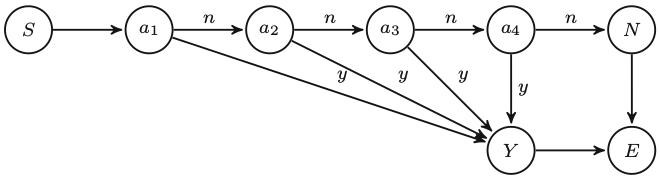
\includegraphics[scale=0.5]{imagens/control_flow.png}
\caption{Controle de Fluxo \cite{winikoff2017bdi}.}
\label{fig:control_fluxo}
\end{figure}

Para derivar equações que calculem o menor número de caminhos exigidos de um programa começando em $S$ para chegar em $E$ é necessário descobrir quantos destes caminhos são bem-sucedidos (passando por $Y$) e quantos falharam (passando por $N$). Os autores definiram $p(P)$ como o número de caminhos necessários para cobrir todas as arestas do grafo de fluxo de controle correspondente ao programa $P$, $y(P)$ para os caminhos que vão por $Y$ e $n(P)$ para os caminhos que vão por $N$, então $p(P) = y(P) + n(P)$.

Logo após os autores consideram $P_{1};P_{2}$, onde um subprograma $P_{1}$ é colocado em sequencia com $P_{2}$ Figura \ref{fig:grafop1p2}. O subprograma $P_{1}$ requer $p(P_{1})$ testes para cobrir todas as arestas com $n(P_{1})$ testes levando até a falha e $y(P_{1})$ levando à uma execução com sucesso.

\begin{figure}[ht]
\centering
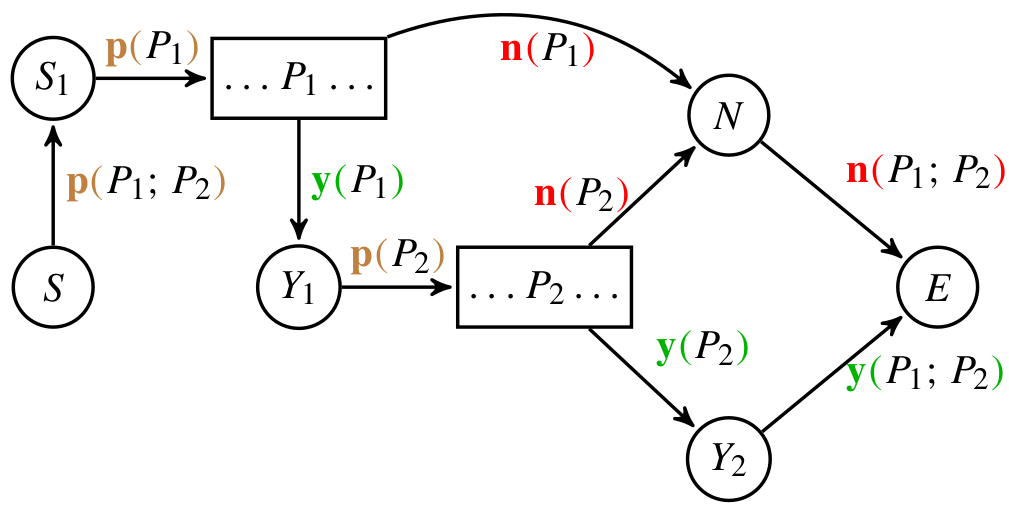
\includegraphics[scale=0.3]{imagens/grafop1p2.png}
\caption{Controle de Fluxo de $P_{1};P_{2}$ \cite{winikoff2017bdi}.}
\label{fig:grafop1p2}
\end{figure}

A partir do exemplo da Figura \ref{fig:grafop1p2} diversas equações são derivadas para os diferentes casos. Estas equações servem para determinar quantos testes são necessários para garantir uma cobertura adequada em relação ao critério todas as arestas. Então os autores implementam as equação em um programa Prolog que calcula os valores de p(p), y(P) e n(P) para qualquer programa BDI. A Tabela \ref{tab:bdirevisited} contém a comparação dos resultados do trabalho anterior dos autores \cite{winikoff2014testability} com os novos resultados encontrados.

\begin{table}[ht]
\begin{threeparttable}
\centering
\caption{Comparação entre os resultados dos trabalhos \cite{winikoff2014testability,winikoff2017bdi}}
\label{tab:bdirevisited}
\begin{tabular}{lllllll}
\hline
                   & \multicolumn{2}{c}{Todos Caminhos}                                            & \multicolumn{4}{c}{Todas Arestas}                             \\ \cmidrule(l){2-7} 
d = j = k = 3      & \multicolumn{1}{c}{n$^{\checkmark}$(g)} & \multicolumn{1}{c}{n$^{\upchi}$(g)} & \multicolumn{2}{c}{p(\textg)} & \multicolumn{2}{c}{p(\cancel{\textg})} \\ \cline{4-7} 
                   &                                         &                                     & Rel.           & Aplic.       & Rel.          & Aplic.        \\ \hline
62 (j = k = 2)     & $6.33 \times 10^{12}$                   & $1.82 \times 10^{13}$               & $141$          & $78$         & $85$          & $64$          \\
363                & $1.02 \times 10^{107}$                  & $2.56 \times 10^{107}$              & $6391$         & $2961$       & $469$         & $378$         \\
776 (j = 2, d = 4) & $ 1.82 \times 10^{157}$                 & $7.23 \times 10^{157}$              & $1585$         & $808$        & $1037$        & $778$         \\
627 (k = 4)        & $3.13 \times 10^{184}$                  & $7.82 \times 10^{184}$              & $10,777$       & $4767$       & $799$         & $642$         \\ \bottomrule
\end{tabular}
    \begin{tablenotes}
      \small
      \item Sendo:  \textit{d} é profundidade da árvore planos-meta, \textit{j} as instâncias de planos aplicáveis e \textit{k} as submetas. 
      Para \textit{Todos Caminhos} n$^{\checkmark}$(g) e n$^{\upchi}$(g) fazem referência ao número de testes que tiveram sucesso e testes que falharam respectivamente. Para \textit{Todas Arestas} o primeiro caso, p(\textg), é para os testes com tolerância a falhas em uso e o segundo caso é para quando a tolerância a falhas está desativada. As colunas com \textit{Rel.} e \textit{Aplic.} são onde os planos associados a um objetivo são, respectivamente, os planos relevantes e os planos aplicáveis
    \end{tablenotes}
    \end{threeparttable}
\end{table}

Este trabalho chegou à conclusão de que o número de teste necessário para \textit{Todas Arestas} é muito menor que para a abordagem de \textit{Todos Caminhos}, encontrando resultados onde é possível realizar os testes na prática. Outra conclusão é que permitir o tratamento de exceções não fez diferença significativa no número de testes como pode ser observado na Tabela \ref{tab:bdirevisited}.

Neste capítulo, trabalhos relacionados ao teste de software em SMA foram apresentados. As abordagens dos trabalhos na grande maioria tratam apenas do nível de agentes ou na testabilidade em nível de agentes. O nível de organização de agentes é uma evolução natural no desenvolvimento de SMA. Logo, estudos avaliando a testabilidade de agentes levando em conta esta dimensão se faz necessária.

